\documentclass[11pt]{aghdpl}
% \documentclass[en,11pt]{aghdpl}  % praca w języku angielskim

% Lista wszystkich języków stanowiących języki pozycji bibliograficznych użytych w pracy.
% (Zgodnie z zasadami tworzenia bibliografii każda pozycja powinna zostać utworzona zgodnie z zasadami języka, w którym dana publikacja została napisana.)
\usepackage[english,polish]{babel}


% Użyj polskiego łamania wyrazów (zamiast domyślnego angielskiego).
\usepackage{polski}

\usepackage[utf8]{inputenc}

% dodatkowe pakiety

\usepackage{mathtools}
\usepackage{amsfonts}
\usepackage{amsmath}
\usepackage{amsthm}

% --- < bibliografia > ---

\usepackage[
    backend=biber,
    style=authoryear-icomp,
    sortlocale=de_DE,
    natbib=true,
    url=false, 
    doi=true,
    eprint=false
]{biblatex}

\usepackage{csquotes}
% Ponieważ `csquotes` nie posiada polskiego stylu, można skorzystać z mocno zbliżonego stylu chorwackiego.
\DeclareQuoteAlias{croatian}{polish}

\addbibresource{bibliografia.bib}

% Nie wyświetlaj wybranych pól.
%\AtEveryBibitem{\clearfield{note}}


% ------------------------
% --- < listingi > ---

% Użyj czcionki kroju Courier.
\usepackage{courier}
\usepackage{float}
\usepackage{listings}
\lstloadlanguages{TeX}

\lstset{
	literate={ą}{{\k{a}}}1
           {ć}{{\'c}}1
           {ę}{{\k{e}}}1
           {ó}{{\'o}}1
           {ń}{{\'n}}1
           {ł}{{\l{}}}1
           {ś}{{\'s}}1
           {ź}{{\'z}}1
           {ż}{{\.z}}1
           {Ą}{{\k{A}}}1
           {Ć}{{\'C}}1
           {Ę}{{\k{E}}}1
           {Ó}{{\'O}}1
           {Ń}{{\'N}}1
           {Ł}{{\L{}}}1
           {Ś}{{\'S}}1
           {Ź}{{\'Z}}1
           {Ż}{{\.Z}}1,
	basicstyle=\footnotesize\ttfamily,
}

% ------------------------

\AtBeginDocument{
	\renewcommand{\tablename}{Tabela}
	\renewcommand{\figurename}{Rys.}
}

% ------------------------
% --- < tabele > ---

\usepackage{array}
\usepackage{tabularx}
\usepackage{multirow}
\usepackage{booktabs}
\usepackage{makecell}
\usepackage[flushleft]{threeparttable}

% defines the X column to use m (\parbox[c]) instead of p (`parbox[t]`)
\newcolumntype{C}[1]{>{\hsize=#1\hsize\centering\arraybackslash}X}


%---------------------------------------------------------------------------

\author{Mateusz Wydmański, Michał Kałduś, Rafał Kwaśnik}
\shortauthor{M. Wydmański, M. Kałduś, R. Kwaśnik}

%\titlePL{Przygotowanie bardzo długiej i pasjonującej pracy dyplomowej w~systemie~\LaTeX}
%\titleEN{Preparation of a very long and fascinating bachelor or master thesis in \LaTeX}

\titlePL{Sprawozdanie z modelowania systemu ofiara-drapieżnik}
\titleEN{}


\shorttitlePL{Sprawozdanie z modelowania systemu ofiara-drapieżnik} % skrócona wersja tytułu jeśli jest bardzo długi
\shorttitleEN{}

\thesistype{}
%\thesistype{Master of Science Thesis}

\supervisor{dr inż. Jakub Porzycki}
%\supervisor{Marcin Szpyrka PhD, DSc}

\degreeprogramme{Informatyka}
%\degreeprogramme{Computer Science}

\date{2016}

\department{Katedra Informatyki Stosowanej}
%\department{Department of Applied Computer Science}

\faculty{Wydział Elektrotechniki, Automatyki,\protect\\[-1mm] Informatyki i Inżynierii Biomedycznej}
%\faculty{Faculty of Electrical Engineering, Automatics, Computer Science and Biomedical Engineering}

\acknowledgements{}


\setlength{\cftsecnumwidth}{10mm}

%---------------------------------------------------------------------------
\setcounter{secnumdepth}{4}
\brokenpenalty=10000\relax

\begin{document}
\nocite{*}
\titlepages

% Ponowne zdefiniowanie stylu `plain`, aby usunąć numer strony z pierwszej strony spisu treści i poszczególnych rozdziałów.
\fancypagestyle{plain}
{
	% Usuń nagłówek i stopkę
	\fancyhf{}
	% Usuń linie.
	\renewcommand{\headrulewidth}{0pt}
	\renewcommand{\footrulewidth}{0pt}
}

\setcounter{tocdepth}{2}
\tableofcontents
\clearpage

\chapter{Wprowadzenie}
\label{cha:wprowadzenie}

$$	\frac{dx}{dt} = \alpha x - \beta x y $$
$$	\frac{dy}{dt} = \delta xy - \gamma y $$

gdzie

\begin{eqwhere}[2cm]
	\item[$x$] liczebność populacji ofiary
	\item[$y$] liczebność populacji drapieżnika
	\item[$\frac{dx}{dt}$,$\frac{dy}{dt}$] przyrost populacji w jednostce czasu
	\item[$t$] czas
	\item[$\alpha$,$\beta$,$\delta$,$\gamma$] parametry opisujące interakcje między populacjami i właściwości populacji
\end{eqwhere}

\noindent Modele ofiar drapieżników są jednymi z najważniejszych elementów składających się na bio- i ekosystemy. Gatunki konkursują, ewoluują, rozprzestrzeniają się dla bolączki poszukiwania pożywienia i możliwości przedłużenia linii garunku. Konkurencja może przyjmować różne formy: drapieżnik-ofiara,wirus-system immulonogiczny, pasożyt-nosiciel, surowiec-konsument, itd. 

\noindent W 1926 słynny Włoski matematyk Vito Volterra zaproponował prosty model opisujący interakcje między ofiarą i drapieżnikiem. Bazuje na kilku założeniach dotyczących środowiska, w którym koegzystują populacje ofiar i drapieżników, to jest:

\begin{itemize}
	\item Ofiara ma zawsze wystarczająco dużo pożywienia.
	
	\item Zaopatrzenie w pożywienie drapieżników zależy wyłącznie od wielkości populacji ofiar.
	
	\item Tempo wzrostu populacji jest proporcjonalne do jej wielkości.
	
	\item Środowisko nie podlega zmianom na korzyść którejkolwiek z populacji, a ewolucja genetyczne jest niekonswekwentna.
	
	\item Drapieżniki mają ograniczony apetyt.
\end{itemize}

\noindent Równania Lotki-Volterry, to para równań różniczkowych I rzędu, nieliniowych.

\noindent Analiza równań mówi nam, że zmiana ilościowa populacji ofiar jest równa jej tempu wzrostu minus  tempo z jaką populacja drapieżników eliminuje ofiary ze środkowiska. Z drugiego zaś biegunu, tempo wzrostu populacji drapieżników jest równoważne tempu wzrostu zasilanym przez dostępność pożywienia minus tempo ubytku populacji na skutek śmierci naturalnej.

\noindent Portret fazowy modelu Lotki-Voleterry daje interesujące rezultaty.

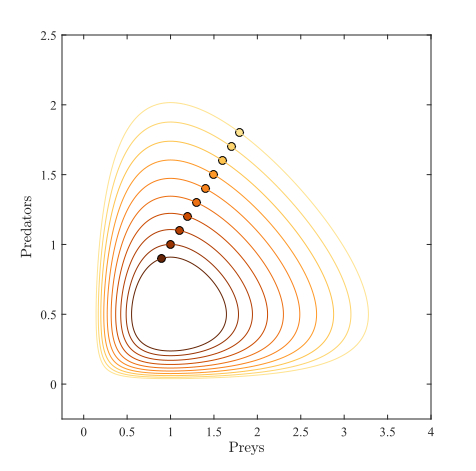
\includegraphics{img/symu}

\noindent Powyższy diagram pokazuje fluktuacje w ilości populacji ofiar i drapieżników. Koła zaznaczona na brzegach zamkniętych powierzchni pokazują warunki początkowe (dla stałych parametrów), gdzie ilości na osiach są rzędu $10^3$. W tym przypadku punktem stałym (populacje obu gatunków są ustalone i nie podlegają zmianom w czasie) jest punkt $(1;0.5)$. 

\noindent W modelu wyraźnie widać, że okres dobrego rozwoju drapiezników przypada gdy populacja ofiar jest duża. Jednakże, poprzez nadmierny rozrost i stopniowe malenie pokładów pożywienia, populacja drapieżników maleje. Wówczas, ofiary nie są na przysłowiowym „celowniku” i mają warunki do rozwoju. Koło się zatoczyło i cykl powtarza się.

\noindent Dla podanego systemu istnieją dwa ekwilibria. Jedno, punkt $(0;0)$, jest równoznaczne wymarciu obu populacji. Taki stan rzeczy będzie się miał  niezależnie od upływającego czasu. Podobnie, drugie ekwilibrium, z obiema populacjami o dodatnich wartościach, jest zależne od początkowych parametrow określających właściwości populacji ofiar i drapieznika.

\noindent Interesujące z biologicznego punktu widzenia jest stabilność układu dla drugiego ekwilibrium. 

\begin{equation}
\lambda_1=i\sqrt{\alpha\gamma} \quad \lambda_2=-i\sqrt{\alpha\gamma}
\end{equation}

\noindent Linearyzacja modelu wokół interesującego punktu: wartości własne jakobianu dla modelu przy drugim ekwilibrium są czysto urojone. Ten krytyczny punkt jest bifurkacją Hopfa – przy niewielkiej zmianie stabilność systemu zmienia się i pojawiają się rozwiązania okresowe. Warto podkreślić, że I metoda Lapunowa nie rozstrzyga o stabilności punktu równowagi, jeżeli system zlinearyzowany jest jedynie stabilny. \cite{Mit}

\noindent Punkt ustalony jest eliptyczny i na podstawie teorii Kolmongorova-Arnolda-Mosera (KAM), która daje odpowiedź na zachowanie w pobliżu punktów eliptycznych, populacje odchylone od punktu ustalonego będą podlegały oscylacjom z częstością $ \omega=\sqrt{\alpha\gamma} $.

\vspace{1cm}
\begin{figure}[ht]
	\centering
	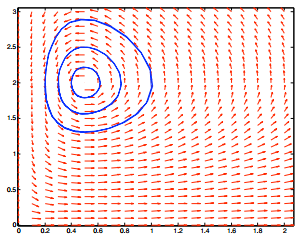
\includegraphics[width=0.6\textwidth]{img/phase}
	\caption{Portret fazowy przedstawionego modelu. Widać oscylujące wokół ekwilbrium rozwiązania i nieograniczony wzrost jednej populacji przy wymarciu drugiej}
\end{figure}














\chapter{Analiza modelu z zachowaniem stadnym}
\label{cha:spatial}

\section{Model matematyczny}

Model matematyczny opisujący zachowania ofiara-drapieżnik:

$$ \frac{\partial X}{\partial t} = rX(1-\frac{X}{K})-\frac{\alpha\sqrt{X}Y}{1+t_h \alpha\sqrt{X}}+d_x \bigtriangledown^2 X $$
$$ \frac{\partial Y}{\partial t} = sY^2+\frac{c\alpha\sqrt{X}Y}{1+t_h \alpha\sqrt{X}}+d_x \bigtriangledown^2 Y $$

gdzie 

\begin{eqwhere}[2cm]
	\item[$X$] liczebność populacji ofiary
	\item[$Y$] liczebność populacji drapieżnika
	\item[$r$] współczynnik przyrostu populacji ofiary
	\item[$K$] zdolność pojemnościowa układu
	\item[$\alpha$] efektywność poszukiwawcza populacji ofiar przez drapieżniki
	\item[$c$] współczynnik żarłoczności drapieżników
	\item[$t_h$] średni czas działania
	\item[$\frac{dx}{dt}$,$\frac{dy}{dt}$] współczynnik dyfuzji odpowiednich populacji
\end{eqwhere}

\noindent W powyższym modelu populacje poruszają się losowo - opisane poprzez model ruchów Browna. Zachowanie zostało uwzględnione w równaniach. Czas działania autor opracowania przyrównał do zera dla uproszczenia rozważań. $\bigtriangledown$ jest operatorem Laplace'a w przestrzeni dwuwymiarowej $R$ = ($R_1$,$R_2$) używanym dla wyrażenia ruchów populacji.

\section{Stabilność}

\noindent Interesuje nas stabilność tego systemu. Z biologicznego punktu widzenia jesteśmy zainteresowani w studiach zachowania koegzystujących populacji ofiar i drapieżnika. Niech punkt równowagi będzie postaci (x*,y*), gdzie obie populacje mają dodatnie wartości i żadna nie wymarła. Okazuje się, że takie ekwilibrium istnieje.

$$ x* = 1 - \frac{c}{s}, \quad y* = \frac{c}{s}\sqrt{x*}$$

\section{Bifurkacje}

\noindent Wraz ze zmianą niektórym parametrów (c,s) struktura jakościowa modelu może się dramatycznie zmienić. Bifurkacją nazywamy skokową zmianę właściwości modelu matematycznego przy niewielkiej zmianie parametrów. Przykładem może być liczba Reynoldsa, ważna w mechanice płynów bezwymiarowa liczba, która oszacowuje występujący podczas ruchu płynu stosunek sił bezwładności do sił lepkości. Przez zmianę tego parametru ruch płynu może zmienić się z laminarnego w falowy albo turbulentny.

\noindent W systemach reakcji-dyfuzji wyróżniamy dwa typy bifurkacji - Hopfa i Turinga. Interesującą bifurkacją jest ta druga, prowadzi bowiem do stanu, gdzie na całej modelowanej przestrzeni pojawiają wzory. W dwóch wymiarach są nimi zwykle heksagony lub figury o pasiastej aparycji.

\noindent W modelu możliwe jest wyznaczenie relacji między parametrem $s$ i $c$, dla którego wartość parametru $s$ będzie wartością krytyczną dla bifurkacji Hopfa i Turinga.

\begin{figure}[h]
	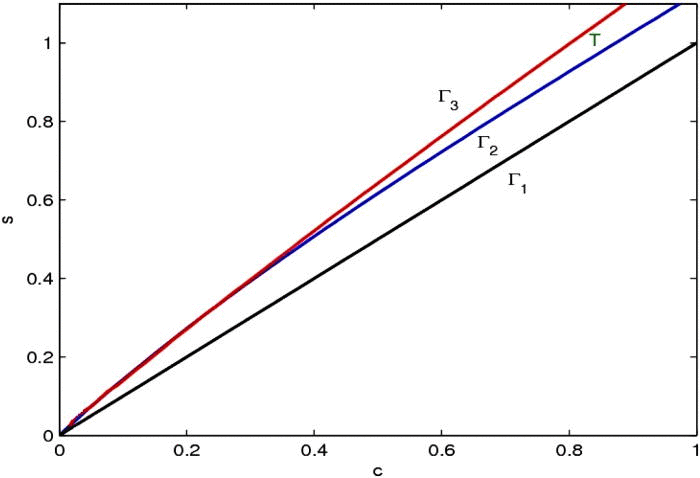
\includegraphics[width=\textwidth]{img/plane}
	\centering 
	\caption{Przestrzeń Turinga oznaczona jako T dla $\delta=10$. $\tau_1$,$\tau_2$,$\tau_3$ są kolejno są liniami bifurkacji Turinga, Hopfa, i ekwilibrium egzystencji.}
\end{figure}

\clearpage

\section{Symulacje}
\noindent Istotnie, interesujące zachowania ujawniają się dla wyznaczonych parametrów. Widoczne są różne kategorie wzorów na skutek bifurkacji Turinga dla różnych wartości parametrów w przestrzeni Turinga.


\begin{figure}[ht]
	\centering
	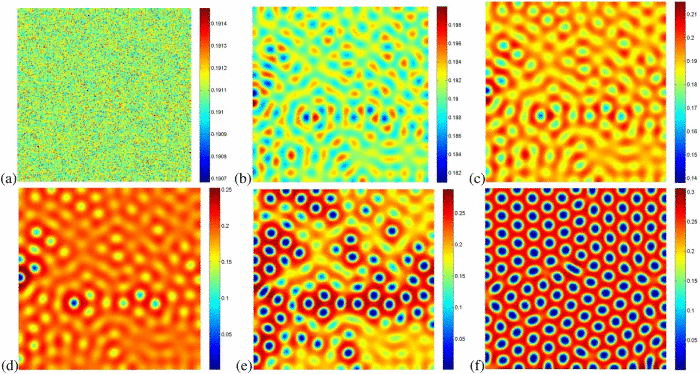
\includegraphics[width=0.6\textwidth]{img/3}
	
	\vspace*{\floatsep}% http://tex.stackexchange.com/q/26521/5764
	
	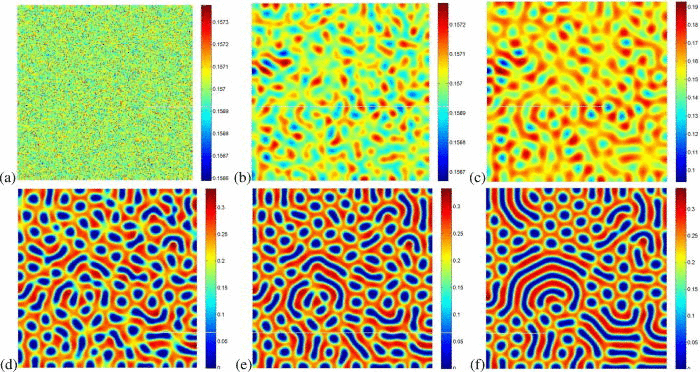
\includegraphics[width=0.6\textwidth]{img/2}
	
	\vspace*{\floatsep}% http://tex.stackexchange.com/q/26521/5764
	
	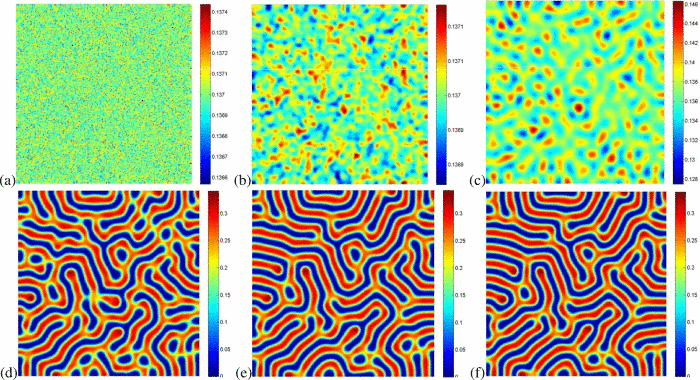
\includegraphics[width=0.6\textwidth]{img/1}
	
	\caption{Ewolucja zagęszczenia populacji ofiar w funkcji czasu}
\end{figure}


\chapter{Automaty komórkowe}

\section{Zagadnienie automatów}

\noindent Ciekawym zagadnieniem dotyczącym dzisiejszej informatyki jest symulacja  różnego rodzaju zjawisk, wydarzeń i populacji. Interesującą właściwością symulowanych modelów jest złożoność zachowań przy nakreśleniu prostych reguł działania. Na myśl nasuwa się pytanie: jakie zachowania będą przejawiały systemy zamodelowane bardziej wyrafinowanymi zasadami. Ograniczenia systemu w połączeniu z modelami matematycznymi oraz mocą obliczeniową komputerów mogą dać ciekawe rezultaty, których moglibyśmy nie przewidzieć. Utworzenie odpowiedniego modelu i wybranie odpowiednich warunków początkowych, pozwala nam też sprawdzić jak zachowa się dany system.
\noindent W celu zrealizowania podanego systemu jako program komputerowy na pomoc przychodzą nam automaty komórkowe. Dzięki prostocie zasad ich działania w bardzo krótkim czasie jesteśmy w stanie stworzyć prosty mechanizm, który będzie symulował rozwój populacji zwierząt. Stopniowo wprowadzając zasady działania populacji, od najprostszych jakimi jest poruszanie się i zdobywanie pokarmów, po te bardziej skompilowane jakimi jest rozmnażanie, uciekanie przed drapieżnikami czy polowanie na inne zwierzęta. Naszą uwagę przykuł fakt jak prosty jednowymiarowy automat komórkowy o prostych zasadach funkcjonowania może, przy niewiele różniących się od siebie regułach, dać zupełnie inny obraz wynikowy. Należy też zauważyć, że najwięcej funkcjonalności automatów komórkowych możemy znaleźć analizują właśnie jednowymiarowe  automaty. Tutaj definiujemy komórke oraz jej sąsiednie komórki, które znajdują się w pewnej odległości od niej. Dzięki temu jesteśmy za pomocą funkcji przejścia wyznaczyć następny stan danej komórki. 
\noindent Zaczniemy od tablicy jednowymiarowej i oznaczymy sobie dwa stany: 1 jako komórkę żywą, 0 jako komórkę  martwą, a jako sąsiadów przyjmiemy tylko te komórki,które znajdują się bezpośrednio przy niej. Ustalimy też, że następny stan będzie zależał bezpośrednio od stanu samej komórki oraz stanu sąsiadów. Wybierzemy też przejścia takie jak na tablicy.

\begin{table}[h!]
\centering
\begin{tabular}{ |c|c|c|c|c|c|c|c| } 
	\hline
	111 & 110 & 101 & 100 & 011 & 010 & 001 & 000\\
	0 & 0 & 1 & 0 & 0 & 1 & 1 & 0 \\
	\hline
\end{tabular}
\label{table:1}
\end{table}
\clearpage

\begin{figure}[ht]
	\centering
	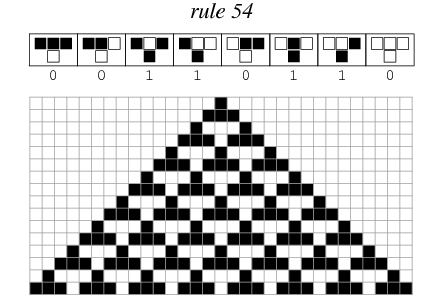
\includegraphics[width=0.8\textwidth]{img/triangle}
	\caption{rezultat wykonania operacji wedle tablicy powyżej}
\end{figure}

\section{Implementacja automatu}

\noindent Modelowanie populacji drapieżnik-ofiara za pomocą automatów komórkowych jest złożoną operacją. Każda komórka to zbiór stanów poszczególnych osobników. Każdy następny stan bazuje na poprzednim oraz na stanach sąsiadów.

\noindent Autorzy książki "A predator-prey model based on fully parallel cellular automata" przeprowadzi symulację na podstawie populacji wilków i owiec. Udało im się znaleźć trzy możliwe stany, do których będzie dochodził system. Są nimi:

\begin{itemize}
	\item współistnienie obu gatunków,
	\item rozwijanie się populacji ofiar,
	\item wyginięcie obu gatunków
\end{itemize}

\noindent Te stany zależały od ilości pożywania dla ofiar, czasu po jakim zwierzęta były wstanie się rozmnażać oraz sposobem opiekowania się na młodymi. Największym problemem z jakim spotkali się twórcy było to, że drapieżnik podczas polowania mógł zabić klika ofiar. Sposobem na poradzenia sobie  z tego typu zjawiskiem było wprowadzenie specjalnego sposobu doboru sąsiedztwa, które nie występowała w innych  automatach, a pozwala blokować możliwość zabicia wszystkich ofiar.  Dodatkowo dyskutowali też jaki wpływ na rozwoje populacji będą mieć takie czynniki jak zagęszczenie oraz mutacje poszczególnych gatunków. Zastanawiali się też jakie wtedy stany może osiągnąć taki automat.
\chapter{Równania Lotki-Volterry dla konkurencji}

\section{Model matematyczny}

\noindent Rozważając temat modelowania populacji za pomocą równań logistycznych warto poruszyć temat modelów uwzględniających również konkurencję o pożywienie i ogólnie system z wielogatunkowymi poziomami troficznymi.

\noindent W odpowiedzi przychodzi układ równań w formie podobnej do klasycznych, modelujących relacje ofiara-drapieżnik. Oparte są na bazie równań logistycznych postaci $\frac{d}{dx}f(x) = f(x)(1-f(x))$.  W przypadku standardowego układu Lotki-Volterry przypadkiem bazowym był wzrost wykładniczy.

\noindent Przypadek zająca i owcy mógłby zostać opisany następującym układem równań:

$$\frac{dN_1}{dt}=N_{1}r_{1}\left(1-\frac{\left({N_{1}+\alpha _{{12}}N_{2}}\right)}{K_1}\right)$$
$$\frac{dN_2}{dt}=N_{2}r_{2}\left(1-\frac{\left({N_{2}+\alpha _{{21}}N_{1}}\right)}{K_2}\right)$$

\begin{eqwhere}[2cm]
	\item[$r_1,r_2$] wzrost per capita członków poszczególnych populacji 
	\item[$\alpha_{nm}$] współczynnik konkurencji jednostki z populacji $m$ na jednostkę z populacji $n$
	\item[$K_1,K_2$] zdolność pojemnościowa układu dla poszczególnych populacji
\end{eqwhere}

\noindent Założeniem logistycznego modelu jest to, że liczba potomstwa per rodzic maleje liniowo ze wzrostem populacji tej populacji.

\noindent Włączając w to konkurencję innego gatunku, liczba potomstwa na rodzica zależy nie tylko od populacji pierwszej, ale również od populacji drugiej.

\newpage

\begin{figure}
	\centering
	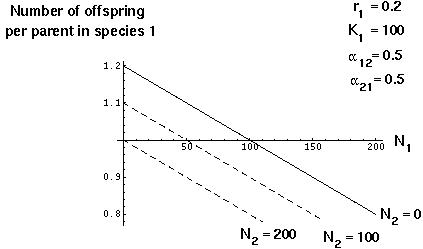
\includegraphics[width=\textwidth]{img/Fig1}
	\caption{Liczba potomków na dorosłego osobnika w funkcji parametrów}
\end{figure}

\section{Właściwości modelu}

\begin{itemize}[itemsep=0em]
	\item jeśli $\alpha_{12}$ wynosi zero, wtedy dynamika gatunku pierwszego będzie przedstawiona równaniem logistycznym (sigmoidalny wykres) 
	
	\item analagicznie dla $\alpha_{21} = 0$
	
	\item jeśli $\alpha_{12} < 0$ to populacja druga zwiększa liczbę surowców dostępnych dla populacji pierwszej
	
	\item jeśli oba współczynniki $\alpha_{12},\alpha_{21} = 0$ to relację między populacjami nazywamy mutualizmem
	
	\item jeśli $\alpha_{12}$ albo $\alpha_{21}$ jest równe zero (albo bardzo blisko zera), to mówimy że populacje są w relacji komensalizmu
	
	\item jeśli tylko jeden ze współczynników jest ujemny, a drugi dodatni, to mówimy, że populacje są w relacji pasożytnictwa
	
	\item jeśli oba współczynniki są dodatnie to populacje ze sobą konkurują
	
\end{itemize}

\section{Symulacje dla dodatnich współczynników}

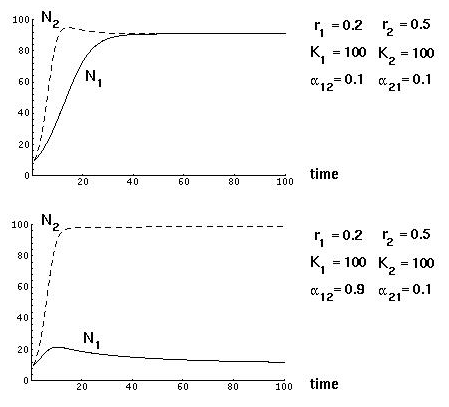
\includegraphics{img/Fig2}

\noindent Jeśli $\alpha_{12}$ i $\alpha_{21}$ są małe, to obie populacje osiągają ekwilibrium w pobliżu odpowiedniej pojemności systemu. Jeśli $\alpha_{12}$ jest znacznie większe od $\alpha_{21}$ (gatunek drugi ma większy impakt na liczebność gatunku pierwszego niż odwrotnie), wtedy liczebność gatunku pierwszego jest utrzymywana na niskim poziomie spowodowanym wyższością konkurencyjności drugiego gatunku.

\noindent Do stworzenia stabilnego ekosystemu wszyste wartości własne macierzy $a_{ij}$ muszą być dodatnie. Duże systemy Lotki-Volterry mogą osiągnąć stabilność jeśli współczynniki konkurencji $\alpha_{ij}$ mogą ewoluować zgodnie z naturalną selekcją (\cite{Kon} i \cite{Ack})
 \chapter{Proponowany model zjawiska}

\section{Cele modelu}
Celem modelu jest zasymulowanie rozwoju populacji zwierząt. Stworzony przez nas program pozwala na zasymulowanie populacji modelu drapieżnik-ofiara w postaci :
\begin{itemize}
	\item jednego gatunku ofiary i  jednego gatunku drapieżnika, który żywi się ofiarą
	\item jednego gatunku ofiary,  drapieżnika żywiącego się ofiarami oraz drapieżnik drugiego stopnia żywiącego się zarówno ofiarami jak i drapieżnikami, lecz preferującemu drapieżniki.
\end{itemize}
 
Zwierzęta mogą poruszać się po zadanym obszarze nie opuszczając go. 

Gdy osoba rozpocznie symulacje może na bieżąco wyświetlać informacje na temat liczby iteracji, ilości populacji każdego z gatunków. Dodatkowo przedstawiony jest widok mapy migracji zwierząt.

System modeluje zachowanie 

\section{Działanie algorytmu} 
W pierwszym etapie działania programu generowanie są populacje zadanych gatunków. Stworzone populacje są rozmieszczane losowo na mapie w ilości uzależnionej od zadanych przez nas współczynników. Następnie na każdym z pól tworzona jest ilość pożywienia dla ofiar, czyli rośliny. 

Po inicjalizacji modelu rozpoczyna się główna część symulacji. W każdej iteracji każde zwierzę obejmuje jakąś strategię działania.
\begin{enumerate}
\item Wspólne na wszystkich zwierząt
	\begin{itemize}
		\item Kopulacja
		\item Wydawanie na świat potomstwa
	\end{itemize}
\item Dla ofiar
	\begin{itemize}
		\item Poszukiwanie i spożywanie roślin
		\item Ucieczka przed drapieżnikami
		\item Odpoczynek
	\end{itemize}
\item Dla drapieżników
	\begin{itemize}
		\item Polowanie na ofiary
		\item Ucieczka przed drapieżnikami drugiego stopnia
	\end{itemize}
\item Dla drapieżników drugiego stopnia
	\begin{itemize}
		\item Polowanie na ofiary i drapieżników
	\end{itemize}
\end{enumerate}

Poszczególne zachowania uzależnione są od aktualnego stanu danego zwierzęcia oraz jego otoczenia.

\begin{enumerate}
\item Wspólne strategie zwierząt
	\begin{itemize}
		\item Jeżeli samica jest w kluczowym stadium ciąży musi wydać na świat potomstwo.
		\item Jeżeli zwierzę jest zagrożone stara się uciec.
		\item Jeżeli współczynnik głodu jest krytyczny ofiara usiłuje zdobyć pokarm.
		\item Jeżeli współczynnik pożądania seksualnego jest krytyczny i osobnik jest wystarczająco dojrzały rozmnaża się z drugim przedstawicielem swojego gatunku przeciwnej płci na danym polu lub szuka partnera w swojej okolicy.
		\item Jeżeli zwierze ma wszystkie współczynniki w normie, odpoczywa.
	\end{itemize}
	
\item Szczególne dla ofiary
	\begin{itemize}
		\item Jeżeli na polu jest drapieżnik, który poluje na ofiarę stara się uciec z danego pola
		\item Jeżeli współczynnik głodu jest krytyczny ofiara żywi się pokarmem na aktualnym polu lub jeśli pole jest pozbawione roślin ofiara szuka ich w swoim najbliższym otoczeniu.
	\end{itemize}
	
\item Dla drapieżnika
	\begin{itemize}
		\item Jeżeli na jego polu jest drapieżnik drugiego stopnia, drapieżnik stara się przemieścić w dogodniejsze dla siebie miejsce
		\item Jeżeli współczynnik głodu jest krytyczny drapieżnik poluje na ofiarę znajdującą się na jego polu lub szuka jej w swoim najbliższym otoczeniu.
	\end{itemize}
	
\item Dla drapieżnika drugiego poziomu
	\begin{itemize}
		\item Jeżeli współczynnik głodu jest krytyczny drapieżnik drugiego stopnia w pierwszej kolejności stara się upolować drapieżnika, który jest preferowanym gatunkiem. W razie jego braku poluje na przedstawiciela gatunku reprezentowanego przez ofiarę.
	\end{itemize}
\end{enumerate}

Dodatkowo w celu organiczna ekspansji populacji ofiar liczba roślin na mapie jest ograniczona przez współczynniki regeneracji roślin po każdej iteracji. Po każdej iteracji zwiększany jest wskaźnik głodu dla każdego zwierzęcia oraz pożądania seksualnego dla dojrzałych osobników. Zwierzę po spożyciu pokarmów otrzymuje wartość energetyczną zjadanego pokarmu, która obniżka wskaźnik głodu.

\section{Symulacja zjawiska}

\subsection{Narzędzi}
Na potrzeby symulacji została stworzona aplikacja okienkowa, która wizualizuje efekty działania programu.
Do zaimplementowania programu posłużyliśmy się językiem Java, a do wyświetlenia danych użyliśmy biblioteki graficznej JavaFX.
\subsection{Aplikacja}
Poniżej przedstawiamy kilka zrzutów ekranu w takcie działa aplikacji.
\subsubsection{Symulacja dla 2 gatunków}
Poniższe obrazy prezentują zachowanie się aplikacji dla dwóch gatunków zwierząt. Na rysunku \ref{fig:pp1} widać jak ofiary i drapieżniki żyją w pomieszanych stadach (początkowe iteracji), a na rysunku \ref{fig:pp2} widzimy jak uformowały się stada poszczególnych populacji.

\begin{figure}[!htb]
	\centering
	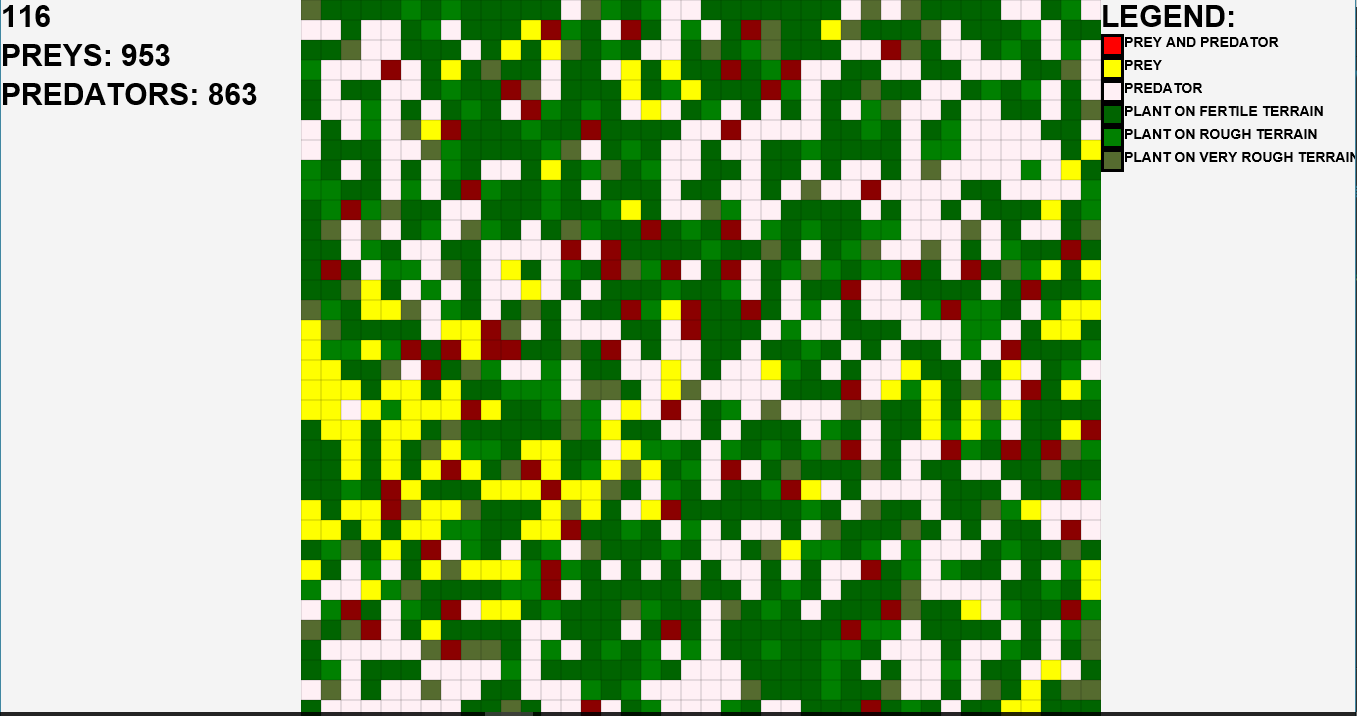
\includegraphics[width=1.1\linewidth]{img/tii1}
	\caption{\label{fig:pp1} }
\end{figure}

\begin{figure}[!htb]
	\centering
	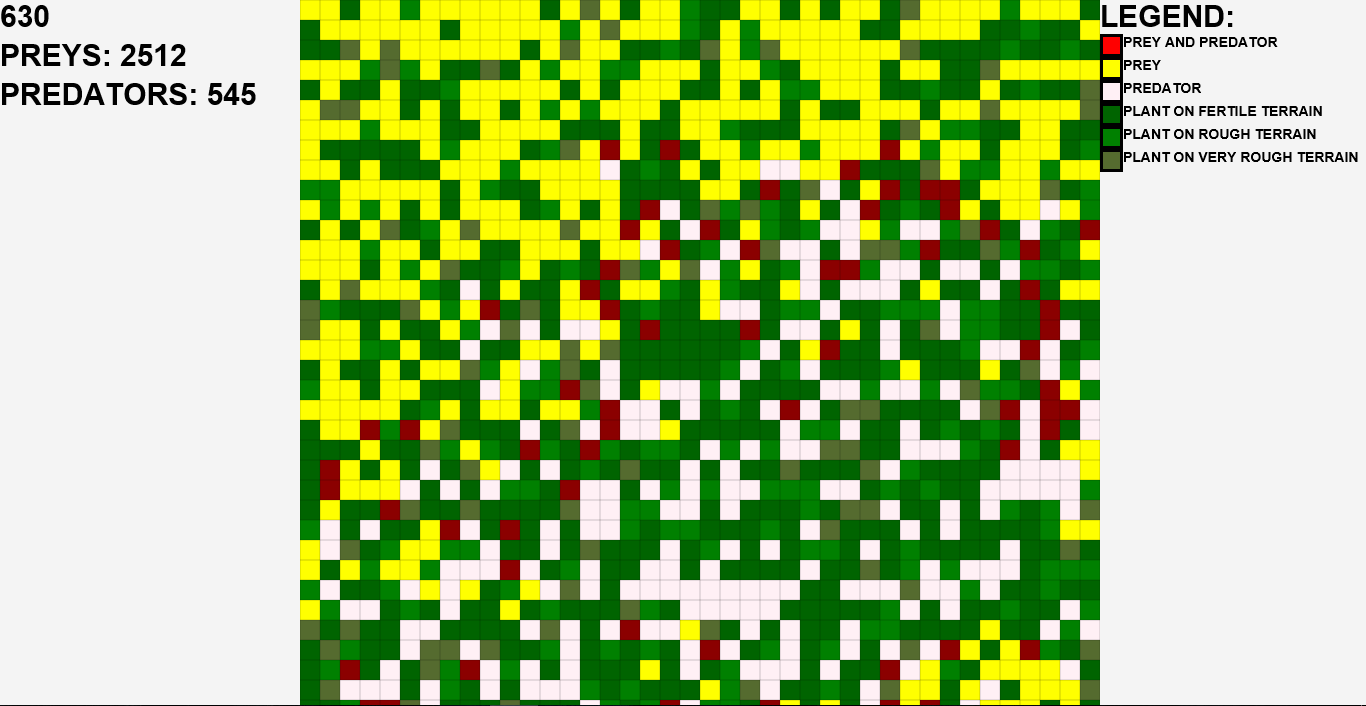
\includegraphics[width=1.1\linewidth]{img/tii2}
	\caption{\label{fig:pp2} }
\end{figure}

\subsubsection{Symulacja dla 3 gatunków}
Poniższe obrazy prezentują zachowanie się aplikacji dla trzech gatunków zwierząt(ofiara, drapieżnik i drapieżnik drugiego stopnia). Na rysunku \ref{fig:pps1} widać jak ofiary i drapieżniki żyją w pomieszanych stadach (początkowe iteracji), a na rysunkach \ref{fig:pps2} \ref{fig:pps3} widzimy jak uformowały się stada poszczególnych populacji.
\begin{figure}[!htb]
	\centering
	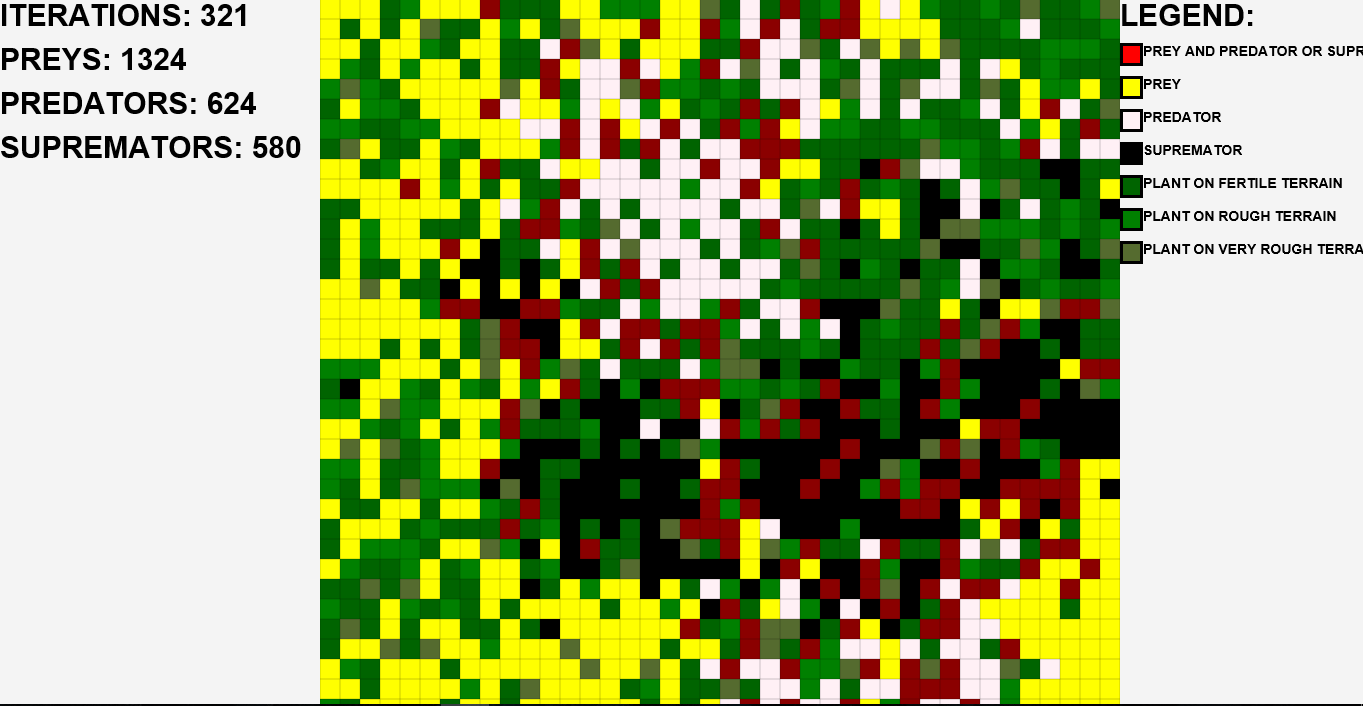
\includegraphics[width=1.1\linewidth]{img/dare}
	\caption{\label{fig:pps1} }
\end{figure}

\begin{figure}[!htb]
	\centering
	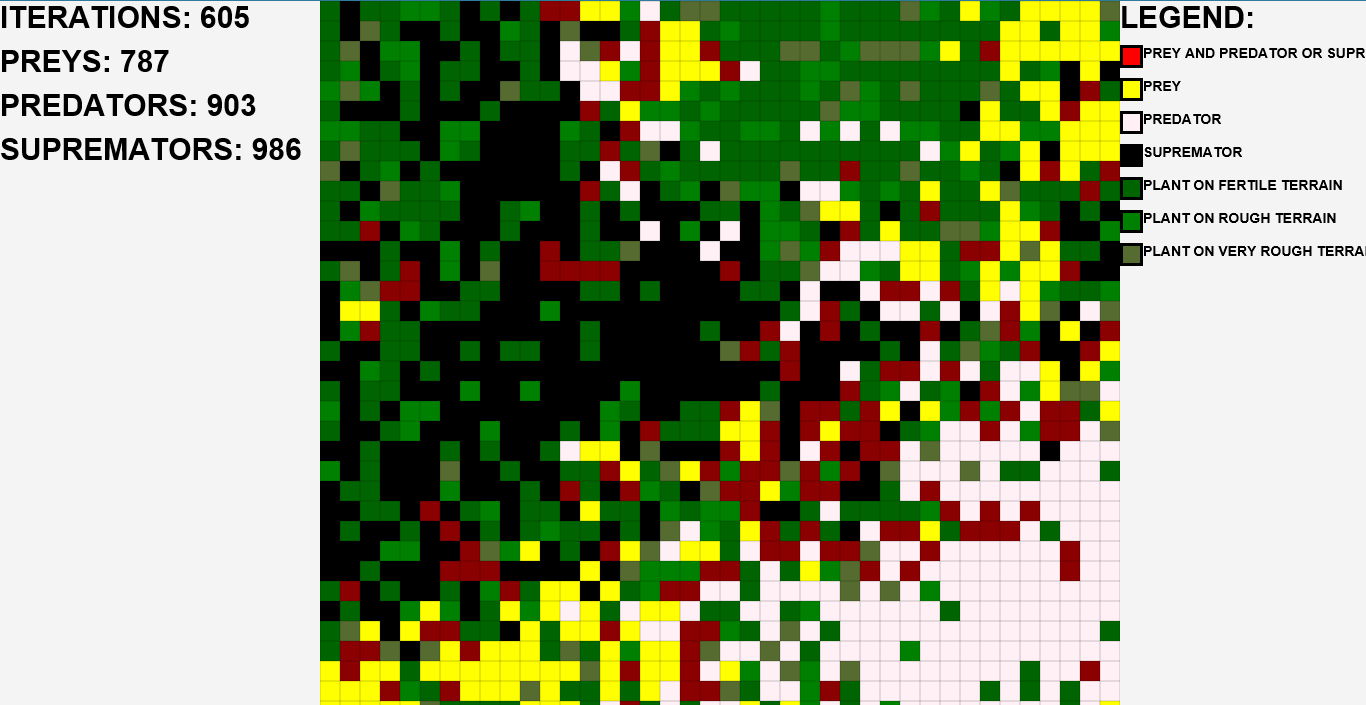
\includegraphics[width=1.1\linewidth]{img/dare2}
	\caption{\label{fig:pps2} }
\end{figure}

\begin{figure}[!htb]
	\centering
	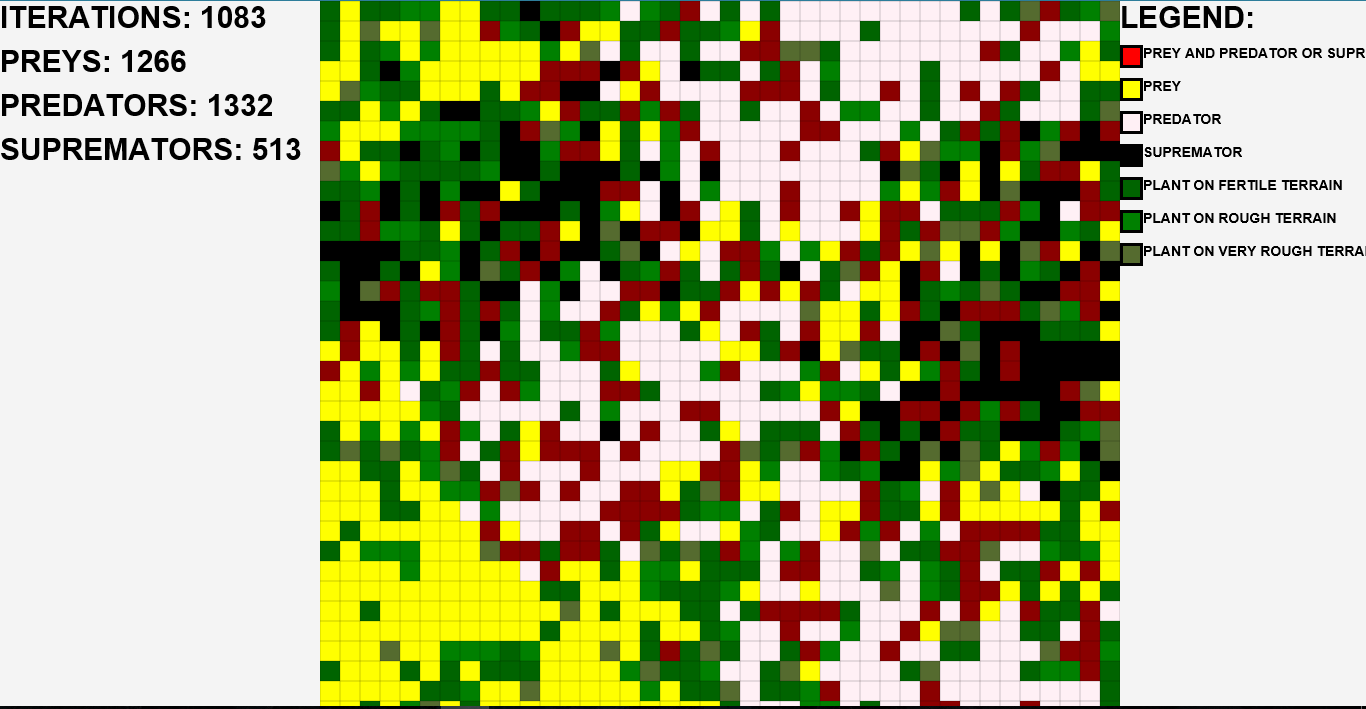
\includegraphics[width=1.1\linewidth]{img/dare3}
	\caption{\label{fig:pps3} }
\end{figure}

 Warto też zwrócić uwagę na to ze życie w większych stadach z dala od swoich ofiar powoduje zagrożenie gatunku i przymus migracji.
 
\newpage
\subsection{Wyniki}

Wyniki kilku symulacji zapisaliśmy do pliku tekstowego, a następnie stworzyliśmy na tej podstawie odpowiednie wykresy. W celu późniejszej możliwości walidacji przyjętego przez nas modelu.
Rysunek 1.1 przestawia wykres zależności ilości drapieżników od ilości ofiar w trakcie próby liczącej 2000 iteracji.
Dodatkowo należy dodać żę wszystkie symulacje uruchamiane były z takimi samymi parametrami, a mimo to otrzymaliśmy inne rezultaty. 
\newpage




\subsubsection{Wyniki dla 2 gatunków- ofiara, drapieżnik}


\begin{figure}[!htb]
	\centering
	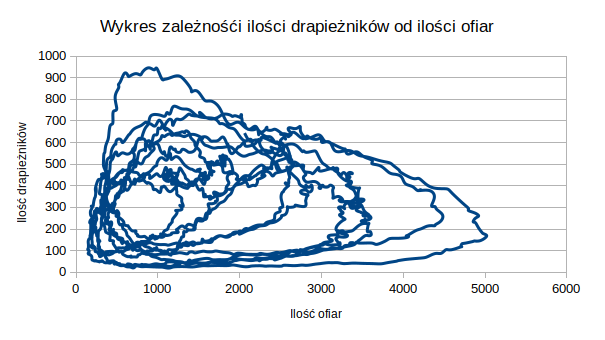
\includegraphics[width=1.1\linewidth]{img/ok11}
	\caption{\label{fig:screen} }
\end{figure}
Powyższy wykres zależności ilość drapieżników od ofiar jest zbliżony do portertu fazowego Lotki-Voltery.
\begin{figure}[!htb]
	\centering
	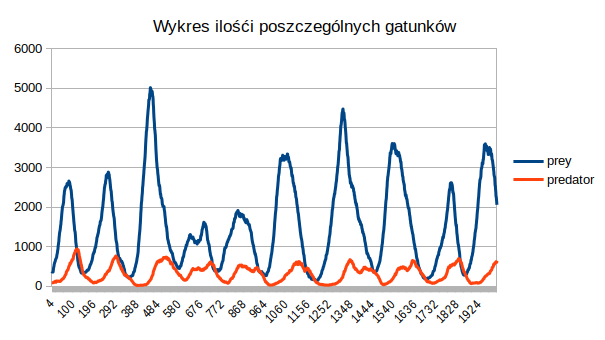
\includegraphics[width=1.1\linewidth]{img/ok1}
	\caption{\label{fig:screen} }
\end{figure}

\begin{figure}[!htb]
	\centering
	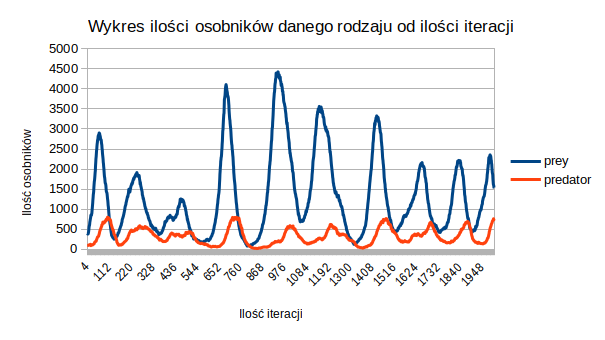
\includegraphics[width=1.1\linewidth]{img/ok2}
	\caption{\label{fig:screen} }
\end{figure}



\begin{figure}[!htb]
	\centering
	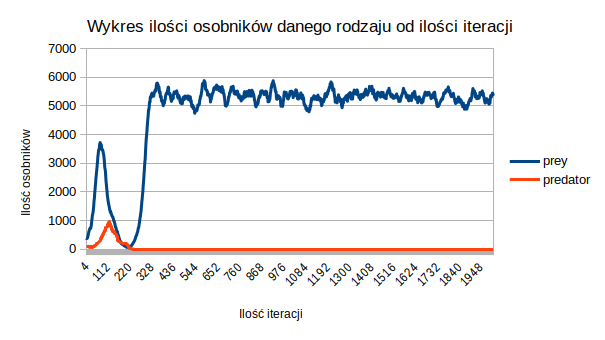
\includegraphics[width=1.1\linewidth]{img/samprey1}
	\caption{\label{fig:screen} }
\end{figure}

\subsubsection{Wyniki dla 3 gatunków- ofiara, drapieżnik i drapieżnik drugiego stopnia}


\begin{figure}[!htb]
	\centering
	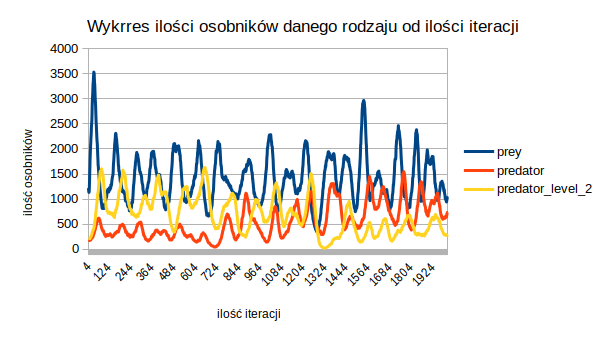
\includegraphics[width=1.1\linewidth]{img/ok3}
	\caption{\label{fig:screen} }
\end{figure}
\begin{figure}[!htb]
	\centering
	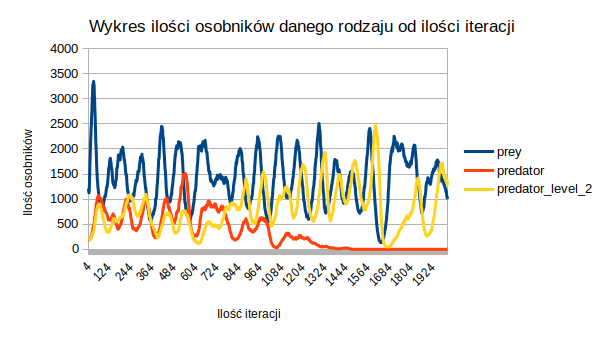
\includegraphics[width=1.1\linewidth]{img/ok4}
	\caption{\label{fig:screen} }
\end{figure}

\begin{figure}[!htb]
	\centering
	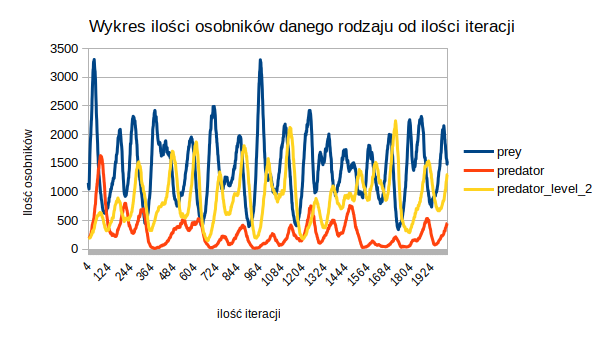
\includegraphics[width=1.1\linewidth]{img/ok5}
	\caption{\label{fig:screen} }
\end{figure}

\section{Wnioski}

Podstawowym wnioskiem jaki zauważyliśmy podczas tworzenia projektu jest to że część współczynników ma ogromny wpływ na działanie i resultat symulacji, a część znikomy. Głównymi współczynnikami naszej symulacją są:
\begin{itemize}
	\item szansa upolowania ofiary
	\item maksymalna możliwa do pokonania odległość w trakcie jednej iteracji
	\item przyrost współczynnika głodu 
\end{itemize}
 Wpływ na wyniki ma też miejsce ulokowania poszczególnych gatunków. Jeżeli już na samym początku drapieżniki otaczają populacje ofiar to  oba gatunki wyginął po upływie kilkunastu iteracji.  

W sytuacji kiedy nasza populacja ofiar w początkowej fazie działania apliakcji da się zagonić w krawędzie, dostępnego pola, podczas pościgu przez gatunki drapieżników i odłączy sie od głównej populacji tylko niewiele stado ofiar istenije bardzo duże prawdopodobieństwo, zę populacje ofiar wyginął, a co skutkuje śmierć populacji drapieżników.

W sytuacji gdy wyginą wszystkie drapieżniki populacja ofiar nie rośnie w nieskończoność, ponieważ istnieje skończona ilość pożywienia dla nich. Wielkość populacja samych ofiar rośnie do pewnej ilości a następnie oscyluje wokół niej. 


\subsection{Nasz model w kontekście istniejących rozwiązań}
Po przejrzeniu dostępnej literatury zarówno polskiej jak również angielskojęzycznej można zauważyć, że jest możliwe znalezienie literatury związanej z automatami komórkowymi oraz z rozwojem populacji zwierząt co sprawiło, ze podczas tworzenia naszego projektu, łatwiej nam było stworzyć odnowieni model. Mimo to częściowy opieraliśmy się na naszej intuicji przy korzystaniu z różnego rodzaju przykładowych prac związanych z automatami, bardzo często odrobinę odbiegającymi od naszego tematu, ale związanymi z automatami co w dużej mierze pomogło nam podczas wykonywania projektu.
Po przetestowaniu naszego projektu korzystając z wielu różnych parametrów wydaje nam się, że całkiem dobrze on przedstawia symulację rozwoju populacji zwierząt w modelu prey-predator i w zupełności spełnia on wszelkie ustalone na początku założenia.

\subsection{Zebranie najważniejszych wyzwań i trudności rozpatrywanego problemu}


Pierwszym napotkanym przez nas problemem było ustawienie maksymalnej możliwej do pokonania odległość w trakcie jednej iteracji tak aby jak najbardziej odzwierciedlało to rzeczywistość, bo długich próbach wybraliśmy odpowiednią wartość, co zostało opisane kilka strony wyżej i również przyniosło bardzo dobre rezultaty.

Zatrzymał nas również dylemat związany z szybką ekspiacją populacji drapieżników, która dosyć szybko zabijała populacje ofiar, a następnie sama ginęła. W celu zniwelowania tej niedoskonałości zmniejszyliśmy szanse upolowania ofiary ze 100 \% na wartość niższą.

Ważnym elementem jest również to, że w zależności od tego czy dany osobnik jest głodny lub spragniony rozmnażania się wykonuje różne czynności, co skutkuje tym, żę polucja migruje oraz zbiera się w grupy w celu tworzenia potomstwa.

Bardzo zależało nam na wykonaniu symulacji, która przedstawi rozwój populacji 3 gatunków co ostatecznie udało nam się uzyskać i jest przedstawione na screenach znajdujących się kilka stron wyżej. To właśnie symulacja rozwoju trzech populacji  sprawdziła czy sposób rezliacji programu jest dobry i czy może być w przyszłości rozszerzalne oraz jest  bardzo cennym osiągnięciem naszego projektu, przedstawiającym jego prawidłowe działanie.

Ostatecznie udało nam się stworzyć aplikację, która symuluje rozwój populacji zwierząt przy wykorzystaniu wiedzy na temat obszaru, na której się ona znajduje i w zależności od panujących warunków następuje rozwój populacji w dobrych warunkach (wszystkie gatunkom udaje się przeżyć, żaden nie dominuje)  jej wymieranie w niekorzystnych warunkach (związanych z wyginięciem ofiar), migracje i ewentualne przemieszczenie się [populacji] w rejony bardziej odpowiednie do rozmnażania się oraz dostępu pokarmu. Warto tu podkreślić, że nie zawsze każda populacja jest w stanie przeżyć, jeżeli znajdzie się ona w obszarze niekorzystnych warunków.




% itd.
% \appendix
% \include{dodatekA}
% \include{dodatekB}
% itd.

\printbibliography

\end{document}
